% Created 2017-03-01 Wed 20:38
\documentclass[10pt]{article}
\usepackage[utf8]{inputenc}
\usepackage[T1]{fontenc}
\usepackage{fixltx2e}
\usepackage{graphicx}
\usepackage{longtable}
\usepackage{float}
\usepackage{wrapfig}
\usepackage{rotating}
\usepackage[normalem]{ulem}
\usepackage{amsmath}
\usepackage{textcomp}
\usepackage{marvosym}
\usepackage{wasysym}
\usepackage{amssymb}
\tolerance=1000
\usepackage{natbib}
\usepackage[linktocpage,pdfstartview=FitH,colorlinks,
linkcolor=blue,anchorcolor=blue,
citecolor=blue,filecolor=blue,menucolor=blue,urlcolor=blue]{hyperref}
\usepackage[margin=2cm]{geometry}
\pagenumbering{gobble}
\usepackage{wrapfig}
\usepackage{multicol}
\setlength\columnsep{20pt}
\author{Alejandro Rodríguez Salamanca - r0650814 - Erasmus}
\date{}
\title{Character recognition with Hopfield networks}
\begin{document}

\maketitle

\begin{multicols}{2}

  \section*{Data preparation}
  Before starting to solve the tasks, the dataset to use must be
  constructed. For this exercise, we are asked to pre-pend the
  lowercase characters of our first and last name to the set of
  capital characters given in \texttt{prprob}. As my name is
  Alejandro Rodriguez, the characters I have to pre-pend are:
  \texttt{a, l, e, j, n, d, r, o, i, g, u, z}. Once this is done,
  it's time to solve the three proposed problems.

  \section*{Task 1: Retrieve the first 5 characters.}
  The first 5 characters of the alphabet are \texttt{a, l, e, j}
  and \texttt{n}, this is, the first five characters that appear in
  my first name and last name. After loading this characters, the
  pixels whose value is 0 must be changed to -1. This has to be done
  because Hopfield networks normally have units that take on values of
  1 or -1 as convention.

  % Image of the characters
  \begin{center}
    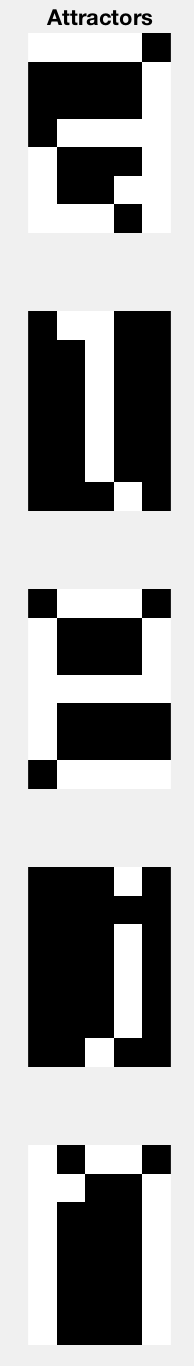
\includegraphics[height=\linewidth]{img/chars1}
  \end{center}

  With this five characters as attractor states, a Hopfield neural
  network is created. Then, three random pixels of each character
  are inverted (from 1 to -1 and vice versa). The objective of this
  inversion is to check if the network is able to reconstruct the
  distorsioned characters.

  \begin{center}
    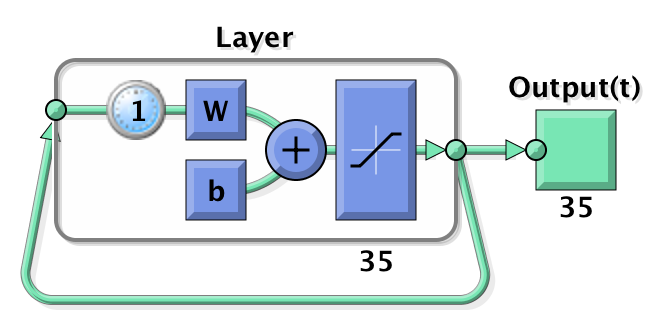
\includegraphics[width=0.7\linewidth]{img/net}
  \end{center}

  Executing the neural network with the noisy characters as input
  shows the following results:

  \begin{itemize}
  \item With a small number of steps: it can be seen that the
    characters are being attracted by the attractor states, but they still
    contain some noise.
    % Image with 2 steps
    \begin{center}
      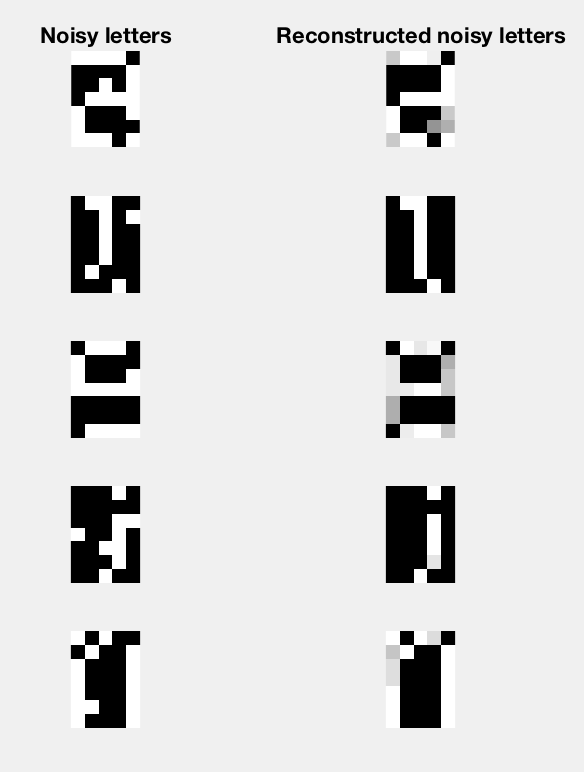
\includegraphics[height=\linewidth]{img/recons1}
    \end{center}
  \item When the number of steps is increased: with just 5 steps, the
    characters are perfectly reconstructed.
    % Image with 5 steps
    \begin{center}
      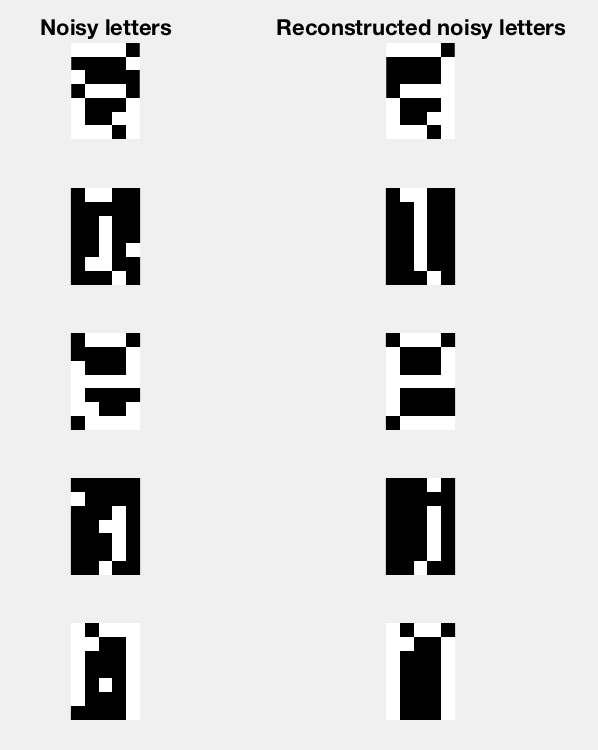
\includegraphics[height=\linewidth]{img/recons2}
    \end{center}
  \end{itemize}

  Sporious patterns are local energy minima that are created during
  training, in addition to the intended target patterns. They are
  activity patterns that have not been explicitly embedded in the
  synaptic matrix, but are nonetheless stable. They are in other
  words "unwanted" attractor states that, by virtue of a finite
  overlap with the "wanted" attractor states, come about as a
  local minimum in the energy function. They can be composed of
  various combinations of the original patterns or simply the
  negation of any pattern in the original pattern set.

  There are three different types of spurious states:

  \begin{enumerate}
  \item For each stored pattern, its negation is also an attractor
  \item Any linear combination of an odd number of stored patterns.
    give rise to the so-called mixture states. Note that Spurious
    patterns that have an even number of states cannot exist, since they might sum up to zero.
  \item for large $p$, we get local minima that are not correlated to
    any linear combination of stored patterns.
  \end{enumerate}

  In this case, the existence of spurious patters is not noticeable.
  According to Hebb rule, a Hopfield network can store up to $0.138N$
  uncorrelated patterns, being $N$ the number of neurons. Replacing
  $N$ by its value in this problem, 35, gives that the uncorrelated
  patterns that can be stored is almost 5, which is the number of
  charaters used in this exercise.

  \section*{Task 2: Critical loading capacity}
  A Hopfield neural network exceed the loading capacity when the number of
  learned patterns over the number of units $p/N$ is greater than the critical
  capacity $\alpha \approx 0.138$.
  First, a number $p = 20$ characters is selected, and the error in the
  reconstruction is calculated as a function of the number of steps used
  to reconstruct the character.

  \begin{center}
    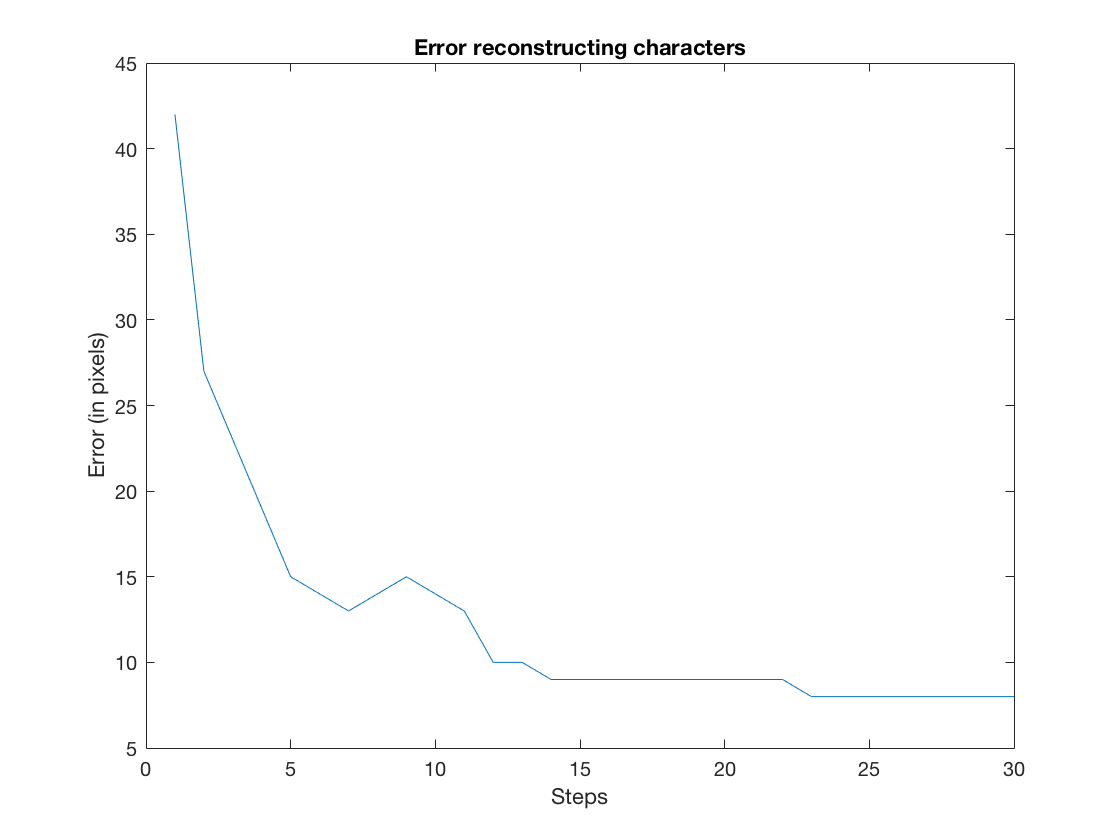
\includegraphics[height=0.8\linewidth]{img/plot_error1}
  \end{center}

  The purpose of this plot is to see how the approximation becomes more
  accurate when the number of steps is increased. Now, let's see what
  happens when the number of characters varies while keeping the number
  of steps fixed at 15.

  \begin{center}
    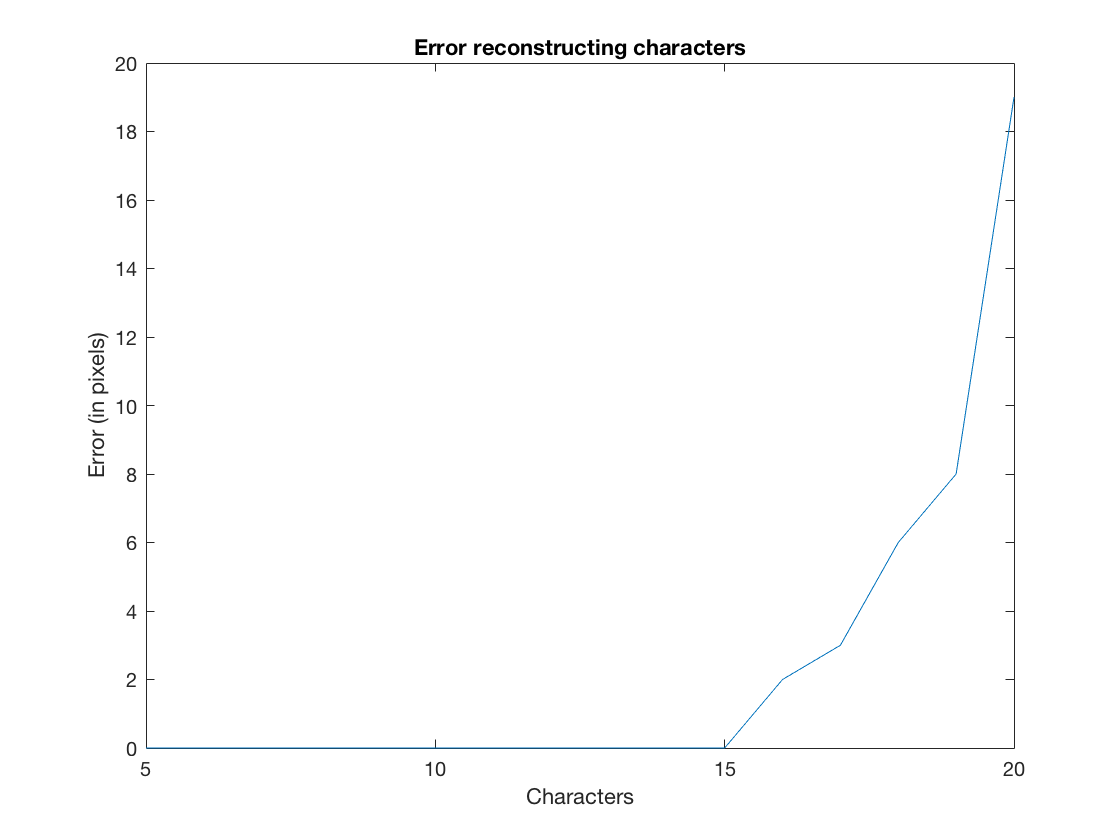
\includegraphics[height=0.8\linewidth]{img/plot_error2}
  \end{center}

  The critical capacity of a Hopfield network, as stated before, is $p/N$,
  where $p$ is the set of patterns to be memorized and $N$ the number
  of neurons. The number of neurons is determined by the number of pixels
  in each image. The dimension of each image is $7 \times 5$, which means that
  the number of neurons of the network is 35.

  Now, the critical capacity can be expressed as $p/35$.

  It can be seen in the previous plot that when the number of patterns
  $p$ has values below 15, there is no error in the reconstruction,
  but when it is increased, an error in the reconstruction appears.

  The loading capacity can be expressed then as $15/35 = 0.428$, which is
  much higher than the one obtained using Hebb-rule.

  This is an interesting phenomena. Nevertheless, it has an explanation. It
  could happen that the spurious states and the real attractors overlap, which
  means that the reconstruction of the character will be correct even if the
  pixel is reconstructed by an spurious state. Hebb rule states that it can be
  stored $0.138N$ uncorrelated patterns, which in this case would be
  $0.138 \times 35 \approx 5$ patterns, as aforementioned. It can be then concluded that
  the charaters are not uncorrelated patterns.    
  
  \section*{Task 3: Retrieve 25 characters}
  % PCA?
  % 
  
  %https://en.wikipedia.org/wiki/Hopfield_network
  %https://cogsci.stackexchange.com/questions/903/spurious-attractors-in-hopfield-networks
  %https://www.quora.com/What-are-spurious-states-in-Hopfield-networks
  % https://www.ncbi.nlm.nih.gov/pmc/articles/PMC4546407/
  % http://www.doc.ic.ac.uk/~ae/papers/Hopfield-networks-15.pdf

\end{multicols}
\newpage

  \section*{Appendix}

\end{document}
